\documentclass{article}
\usepackage[utf8]{inputenc}
\usepackage{geometry}
 \geometry{
 a4paper,
 total={170mm,257mm},
 left=20mm,
 top=20mm,
 }
 \usepackage{graphicx}
 \usepackage{titling}

\title{{\em Einschwingvorgänge} or How to turn on an oscillation}
\author{Manuel Eguia}
\date{October 2024}

\usepackage{fancyhdr}
\fancypagestyle{plain}{%  the preset of fancyhdr 
    \fancyhf{} % clear all header and footer fields
    \fancyfoot[R]{\thedate}
    \fancyfoot[L]{\thepage}
    \fancyhead[L]{Turning on Oscillations}
    \fancyhead[R]{\theauthor}
}
\makeatletter
\def\@maketitle{%
  \newpage
  \null
  \vskip 1em%
  \begin{center}%
  \let \footnote \thanks
    {\LARGE \@title \par}%
    \vskip 1em%
    %{\large \@date}%
  \end{center}%
  \par
  \vskip 1em}
\makeatother

\usepackage{lipsum}  
\usepackage{cmbright}

\begin{document}

\maketitle

\section{Evolution Rules}
We are interested in oscillations for the generation of sound. So we are interested in some magnitude that changes in time in a continuous way but remains bounded. It does not necessarily have to be periodic but it must be continuous because eventually at some point it will be transformed into sound.
We will further consider that this quantity arises from a deterministic system, i.e. the immediate future state of the system is determined by a rule that depends only on the present state. The state of the system is defined by one or more variables that evolve over time, and it is from these variables that we derive the magnitude to be converted into sound. 
Because we assume continuous evolution, defining the concept of "immediate future" requires careful consideration.



\subsection{The simplest case (pure tone)}

\begin{figure} [h]
    \centering
    \resizebox*{17cm}{!}{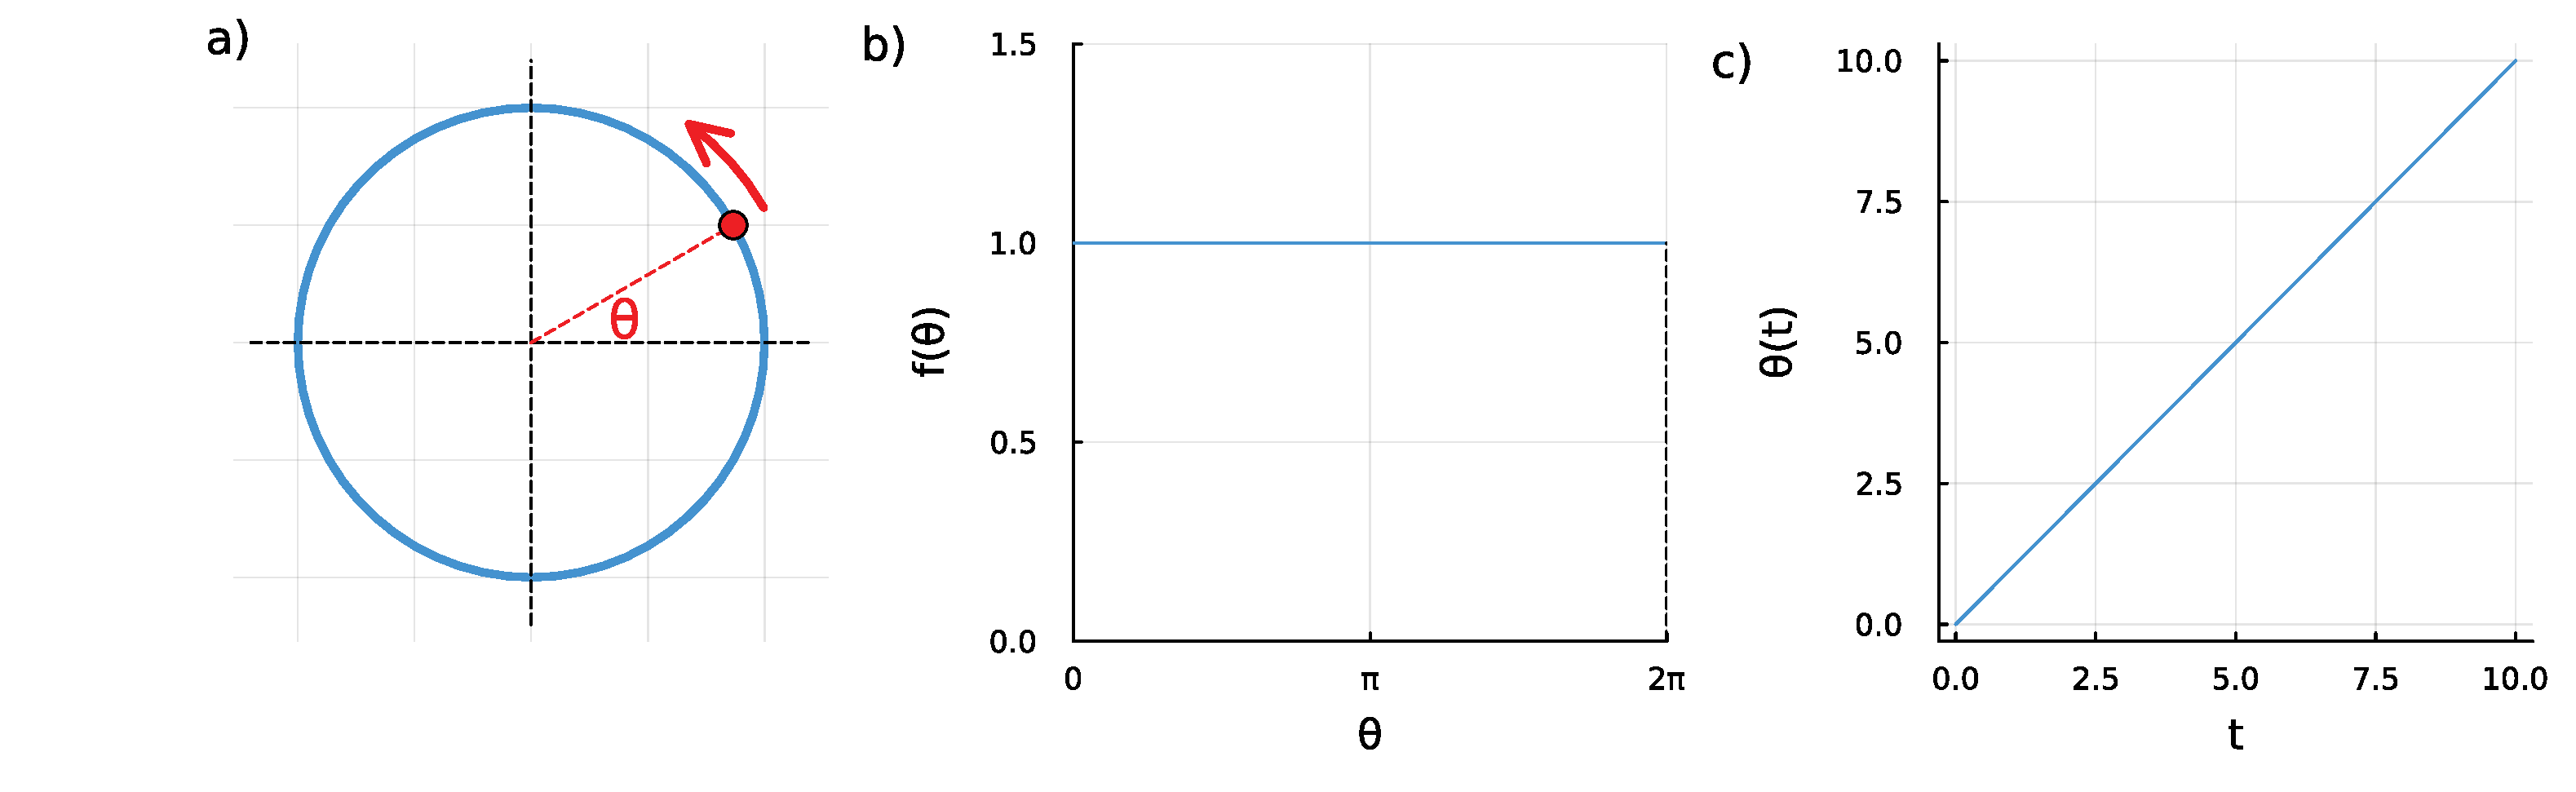
\includegraphics{figure1.eps}}
    \caption{Simplest oscillator given by Equation (1): a) phase space, b) time derivative, and c) time evolution of the variable} 
    \label{fig_pure}
\end{figure}

Let's see an example, perhaps the simplest posible for an oscillator, to understand how this rule must be given. 
Let us consider a system with a state specified by a single angular variable $\theta$. 
We can represent the state of the system as a point on a circle and the magnitude is the angle on the circle as shown in Figure 1.a.
This representation is known as the {\em phase space} of the system and is one where each state is represented by a single point in the space. 
In this case the phase space is one-dimensional but there can be phase spaces of various dimensions and with different topologies (for example a one-dimensional space corresponding to the straight line is topologically different from the circle).
This state of the system $\theta$ is going to vary in time following some deterministic rule and the magnitude that we will convert into sound will be $\cos(\theta)$.

It should not be surprising that at this point the simplest thing that could be proposed as an oscillation is to postulate that the variable of the system grows linearly with time $\theta(t)=\omega t$ as shown in figure 1.c.  Therefore we have at the output a pure tone of frequency $f=\omega/(2\pi)$ and it is clear that the variable $\theta$ represents the phase of this oscillator.

However, notice that in that case we are not giving the rule of evolution of the state of the system but the result of that rule, or the solution of it. 
And there is a problem with this approach being that it is not general and flexible enough. 
For example, it is not always possible to calculate the final result of a given rule. 
Also, the final result also depends on the initial state of the system, while classifying systems by means of their rules will allow us a higher degree of generalization than from their solutions.

As noted, the evolution rule must describe the immediate future state of the system. 
For a continuous system like this, the rule is provided by the time rate of change of our variable $\theta$, which, in this case, corresponds to the slope of the line in Figure 1.c. 
Here, the slope is constant at $\omega=1$, meaning the system evolves at a steady angular rate, independent of its initial state (or initial phase). Figure 1.b displays this constant rate of change, which as we anticipated is always constant. 
It should also come as no surprise that we call the magnitude represented in this graph the angular frequency (or velocity\footnote{The distinction between angular frequency and velocity is subtle and does not apply to the one dimensional case that we are presenting. In general terms the velocity is a vector while the frequency is a scalar magnitude}) of our oscillator.

Let us then for the moment write the evolution rule as: 

[time-varying rate of] $\theta$ = $\omega$

The graphical representation of this rule is given by the graph in Figure 1.b. This means that the rate of change of $\theta$ is uniform, independent of the state of the system. 

Formulating the rule in terms of time-varying rates allows for generalization to scenarios where rates are non-uniform or state-dependent.

\subsubsection{The rule as a differential equation}

We are now ready to give the rule formally using the mathematical concept of {\em derivative}. 
What we wrote earlier as thetime-varying rate of the variable $\theta$ is in fact the definition of the derivative of the variable $\theta$ with respect to time which we will denote with a dot above the variable. 

Our rule is then finally written: 
\begin{equation}
\dot\theta = \omega    
\end{equation}
. 
This is what is known as a differential equation and is the rule that gives the evolution of deterministic systems with continuous variables. 
In general a differential equation for this variable will be written as follows:

\begin{equation}
\dot\theta = f(\theta)    
\end{equation}

where the derivative with respect to time appears always on the left and on the right in general a function $f$ of the state of the system given by our single variable. 
Note that there is no dependence with respect to time, only with respect to the state of the system. 
In the particular case of our simple oscillator this function is constant $f=\omega$ and does not depend on $\theta$. 


\subsection{Non-uniform evolution}

\begin{figure}[h]
    \centering
    \resizebox*{17cm}{!}{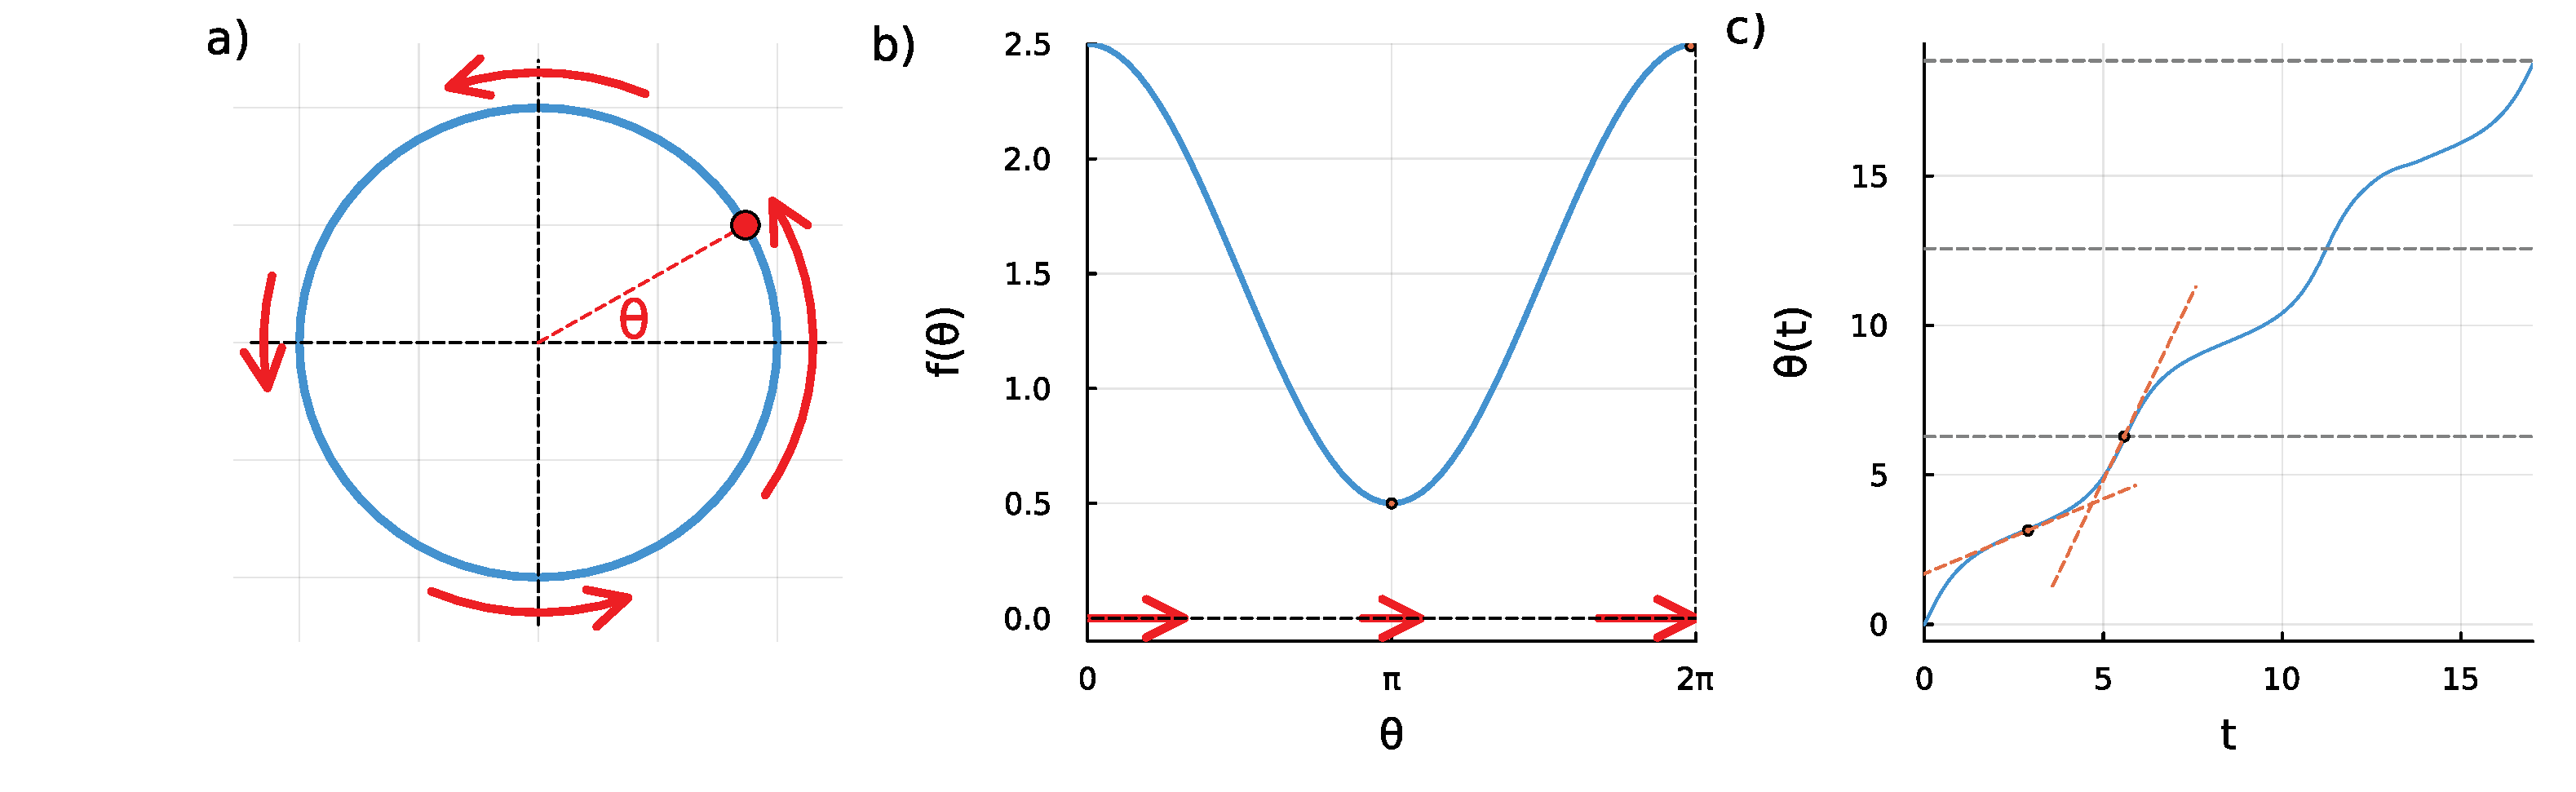
\includegraphics{figure2.eps}}
    \caption{Adler oscillator given by Equation (3) with $\mu=1.5$: a) phase space, b) time derivative, and c) time evolution of the variable} 
    \label{fig_adler1}
\end{figure}

Our next example will be slightly less obvious. 
From now on, we will avoid providing the solution of the variable $\theta$ as a function of time, instead specifying the rate-of-change rule for $\theta$ using a graph like the one in Figure 1.b. or, equivalently as the differential equation for the time evolution of $\theta$.
It is important to note that the states $\theta=0$ and $\theta=2\pi$ represent the same state, so any curve we place in this graph or any function $f(\theta)$ must be periodic in $2\pi$. 
Furthermore, for the moment, we are going to restrict it to be positive for every state, that means that the variable always increases. 

A simple way to create a more interesting scenario than a constant rate of change is to postulate that the angular frequency varies as shown in Figure 2.b. 
Instead of being constant it depends on the angular variable. 
At an angle of 0 (or $2\pi$) has a value of 2.5 while at an angle of $\pi$ it decreases to 0.5.
Before writing our rule as a differential equation, let’s understand what this means in terms of state evolution within the phase space depicted in Figure 2.a. 
The point always moves counterclockwise, but not always at the same speed. On the right side, it moves faster than on the left, and at bottom and top it moves with an intermediate speed, as indicated by the size of the arrows.

Note that we also represent the rate of change on the horizontal axis in the panel b of this Figure using arrows. 
This is exactly as if we were displaying the circle of panel a on the horizontal axis of the graph. 
This qualitative way of representing the rate of change of the state with arrows, which is also known as flow, will be very useful later on.

This could lead to think that the sound result is equivalent to the one obtained by modulating the frequency between 2.5 and 0.5. 
However, it is important to note that unlike traditional FM, this modulation does not occur in a certain way in time, but from a rule that gives the frequency as a function of the phase of the oscillator. 


This distinction is very important and will become evident if we apply the evolution rule and obtain the magnitude transformed to sound, which is shown in Figure 3. 
The waveform obtained is not that of an FM but has a constant frequency and an asymmetric waveform. 
The frequency is constant because once the system returns to the same state after one cycle the behavior will be repeated in exactly the same way. 
And the waveform is asymmetric because the point moves faster in one part of the cycle than in the other.

\begin{figure}[h]
    \resizebox*{6cm}{!}{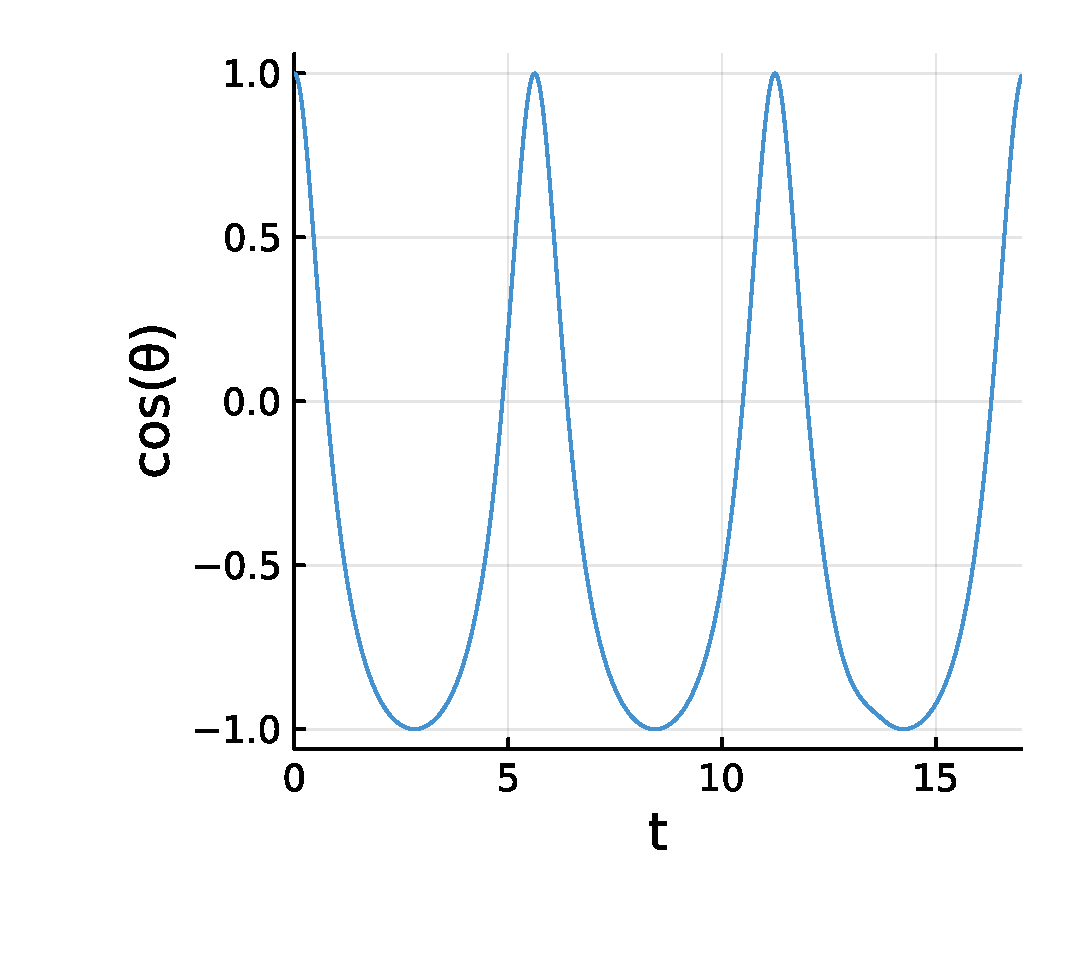
\includegraphics{figure3.eps}}
    \caption{The magnitude to be converted into sound (the cosine of the angle as a function of time) for the Adler's equation (3) with $\mu=1.5$} 
    \label{adler2}
\end{figure}

Let us now write the differential equation governing this system. As before the right hand member $f(\theta)$ indicates the instantaneous angular velocity of the point on the circle as a function of the angle and must be a function of period $2\pi$. 

\begin{equation}
\dot\theta = \mu + \cos(\theta)
\end{equation}

This is known as Adler's equation and is used to model phase locking between oscillators. 
The value $\mu$ represents a {\em parameter} of the system. 
That means, it is a fixed value that once assigned does not change with the evolution of the system. 
For the case we are studying we make $\mu=1.5$ so that $f(x)$ oscillates between 2.5 and 0.5. as shown in Figure 2.b.

This equation cannot be solved in a simple way because unlike an FM we are not specifying the angular frequency as a function of time but instead we are fixing it for each angle value. 
Therefore, as we move on the circle we have to update our angular velocity (the derivative of the angular variable $\theta$) which is equivalent to the slope of the graph of $\theta$ as a function of time shown in Figure 2.c. 
In the graph we also show as an example two instants as orange points where the angle reaches the value $\pi$ and $2\pi$ with their corresponding slopes 0.5 and 2.5. 
If we do this update instant by instant (which is equivalent to integrate numerically our differential equation) we obtain the curve shown in panel c of figure 2: an ever increasing curve, with a slope that varies between 0.5 and 2.5 and that repeats every time it reaches a multiply of $2\pi$ on the vertical axis. 
The cosine of this function in the waveform shown in Figure 3. 
The lower slope parts correspond to the flatter part of the waveform because the point moves slower on the circle and the peaks on the waveform to the faster part on the circle.

At this point we can ask ourselves what would happen with an arbitrary function (as long as it remains periodic and positive). 
We could get very different waveforms but the relationship between $f(\theta)$ and $\cos(\theta)$ is not obvious at all. 
Even more critically, we cannot know in advance the period that the signal obtained will have. 
However, there is something that is intuitive, the greater the value of $f(\theta)$, the faster the point will go along the circle. 
On the other hand, the closer to zero this function gets, the slower the time evolution will become. 

\begin{figure}[h]
    \centering
    \resizebox*{17cm}{!}{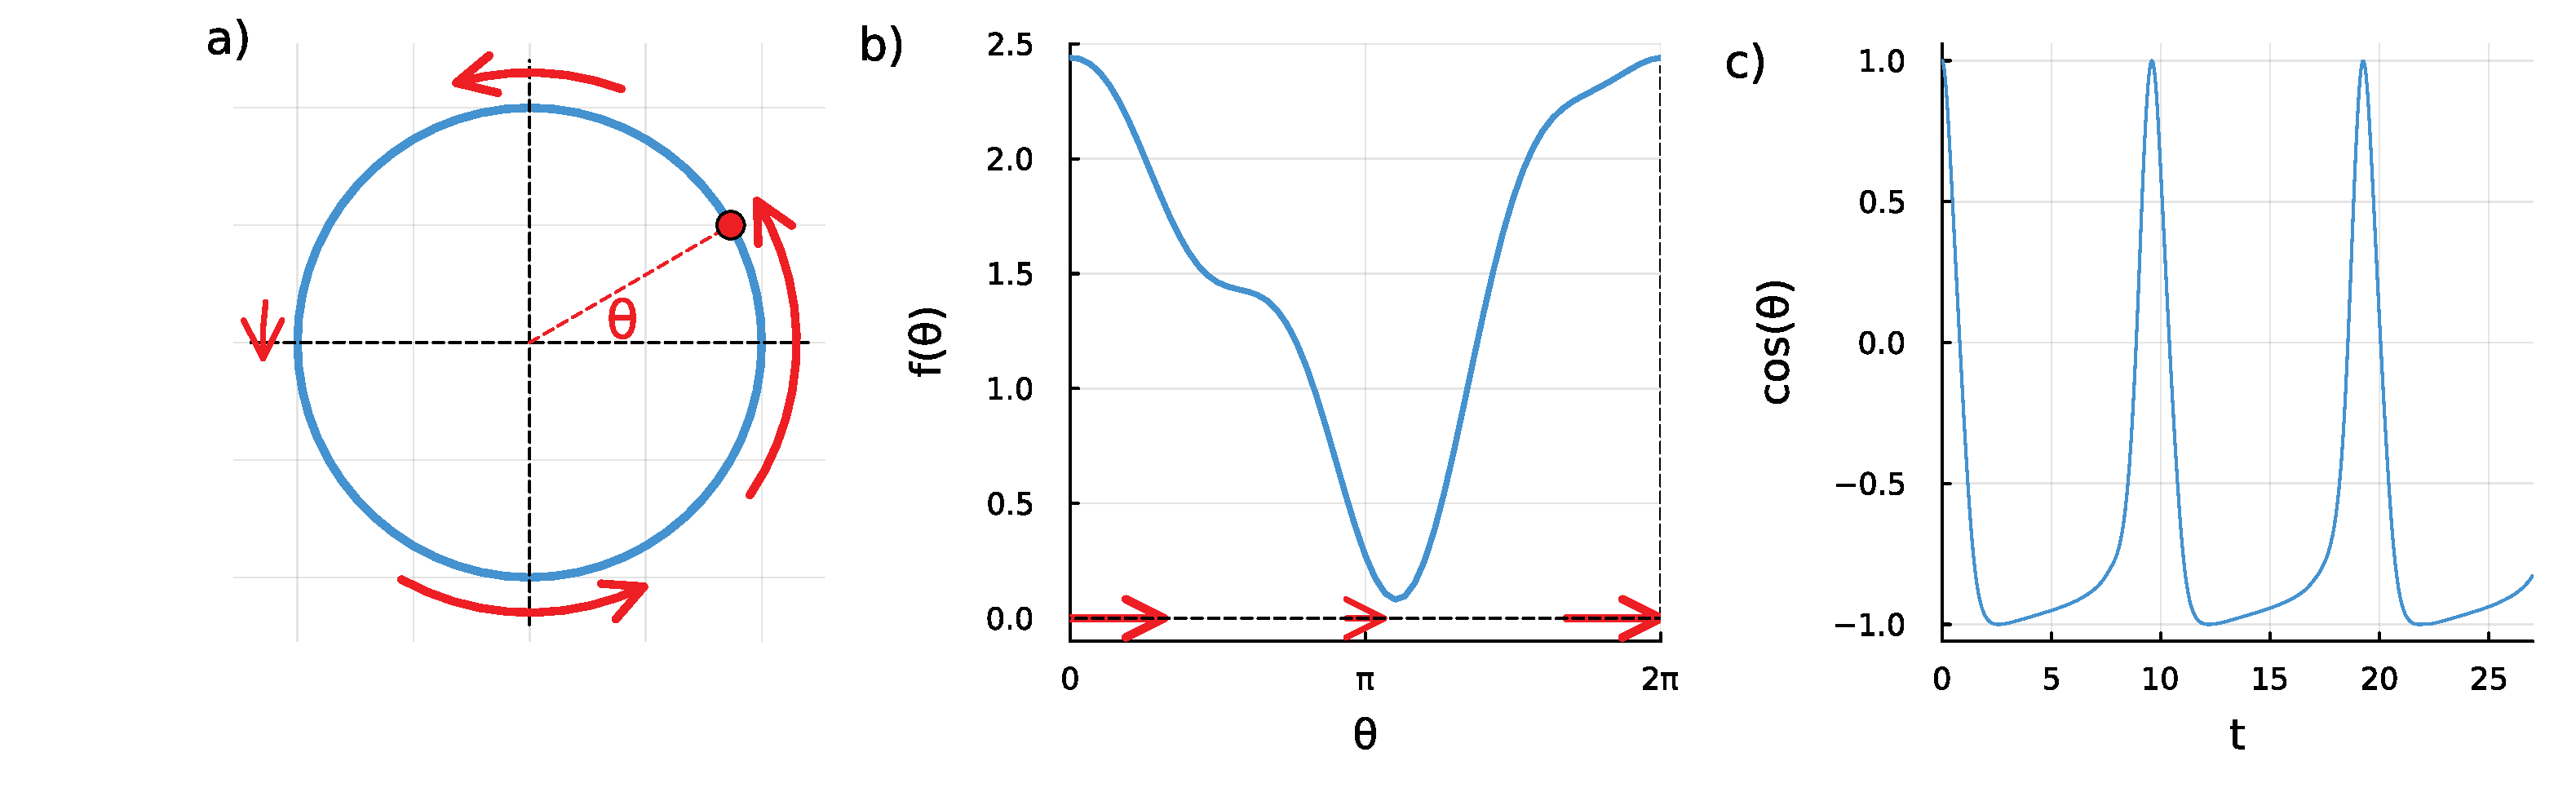
\includegraphics{figure4.eps}}
    \caption{A more general oscillator with an arbitrary periodic positive function $f(\theta)$ displayed in panel b. Panel a and c display the 
    phase space and the time evolution of the cosine of the angle respectively} 
    \label{fig_adler3}
\end{figure}

In Figure 4 we display a more complex function $f(\theta)$ (built with periodic functions but it is not worth to write the differential equation) having a risky approximation to zero for an value of $\theta$ slightly higher than $\pi$ (see panel b of Figure 4). 
In this zone, which corresponds to the left part of the circle in the phase space in Figure 4.a, the motion of the point (or flow) becomes very slow as indicated by the small arrow. 
As expected, this produces a flatter part of the waveform even than in the previous case because the flow slows down much more.




\subsection{The end of an oscillation}



\begin{figure}[h]
    \centering
    \resizebox*{17cm}{!}{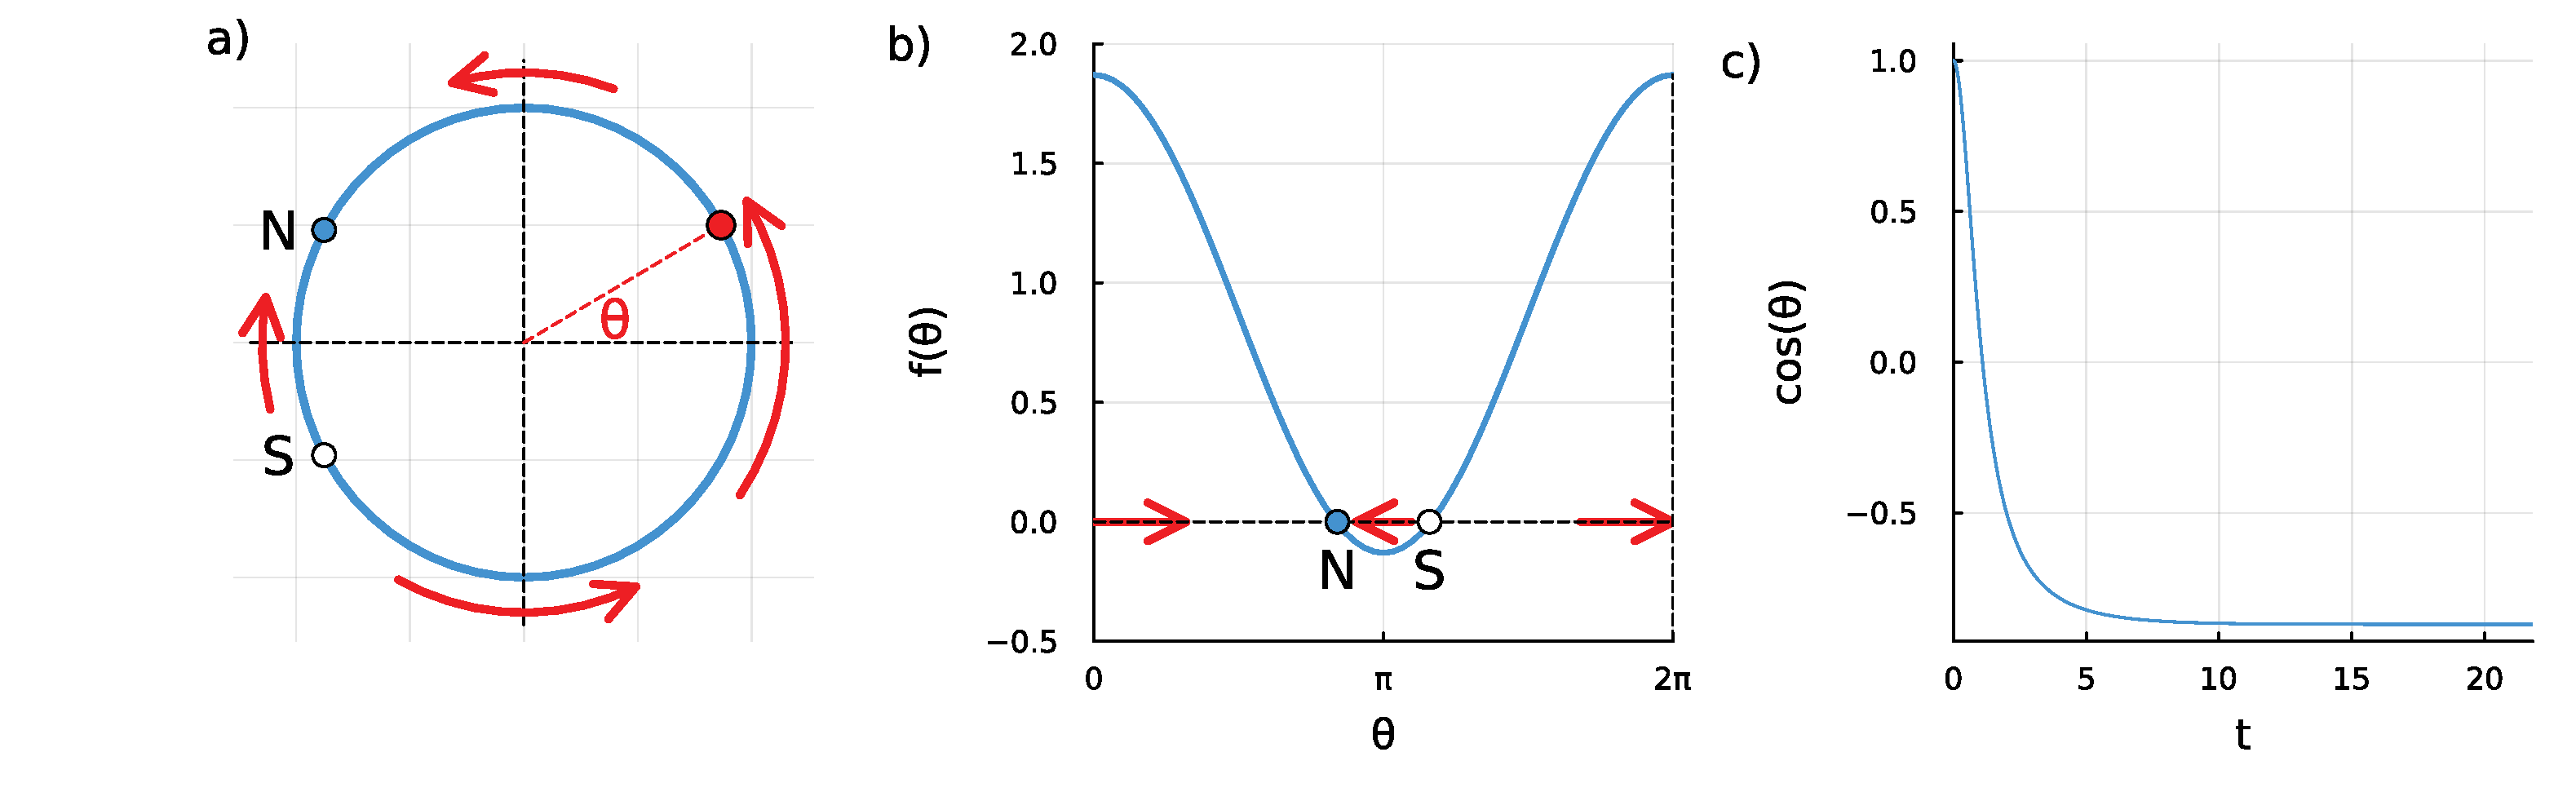
\includegraphics{figure5.eps}}
    \caption{dler oscillator given by Equation (3) with $\mu=0.9$: a) phase space, b) time derivative, and c) the cosine of the angle as a function of time} 
    \label{fig_adler4}
\end{figure}

The next step then is to ask what happens if the function $f(\theta)$ reaches the value zero or crosses the horizontal axis. That is, if we eliminate the requirement that we had put before that this function must be positive for all $\theta$ values. 

Let us return to the original system of the Adler equation but now with a value $\mu=0.9$. This is shown in Figure 5.b. 

Notice that now $f(\theta)$ varies between 1.9 and -0.1 which means that there is a short interval around $\pi$ in which the function is negative. 
This means that in that interval the rate of change of the variable is negative so the point in phase space should go in the opposite direction as indicated by the arrow in Figure 5. 
In other words, unlike before where the value of the variable was always increasing (with greater or lesser rate) now it decreases and the flow moves in the opposite direction at least in part of the phase space.  

The points where the arrow changes direction are indicated as circles with the letters S and N in panels a and b of the Figure 5 and correspond to what are known as fixed points. These fixed points are exactly the points where the function $f(\theta)$ crosses the horizontal axis since there the rate of change is zero and the value remains constant. 
In other words, if the system starts in that state its derivative is zero and therefore does not vary and remains at that value forever which explains the name fixed point. 

Note that there is an important qualitative difference in what happens in a neighborhood of both fixed points. 
In the neighborhood of the fixed point indicated as N the arrows converge to it therefore it is said to be a stable fixed point or Node.  
While in the other fixed point the arrows diverge from it and it is an unstable fixed point. The S stand for Saddle point and the meaning of this term will make sense when we go to a higher dimensional phase space.

What will happen then in the dynamics of this system? 
Any trajectory that starts at an angle where the function is positive will rotate counterclockwise and will approach the node. 
Technically it will never reach it because the flow will become slower and slower around it (it can be shown mathematically that the function of the variable with respect to time corresponds to an exponential decay towards the value of the variable at the node). 
And no matter where we start from we will always tend to the Node, either from the clockwise direction (if we start whitin the shortest arc between N and S) or from the counterclockwise (if we start from any other point). 
This means that there is no more oscillation and we have a decay to a stable fixed point.
This is displayed in Figure 5.c

Let us review then what happened. 
As long as we had a positive function $f(\theta)$ the variable $\theta$ is always growing, with different rates of change, and we have an oscillatory behavior with a waveform with flatter parts in the slower regions and peaks in the faster regions. 
But as soon as the function crosses zero the oscillation disappears. 
So we have not shown how to turn on an oscillation but how to turn it off. 

And this change goes along with the appearance of two fixed points a node and a saddle where before there was a region of very slow flow. 
Later we will see that this qualitative change corresponds to what is known as a {\em bifurcation} of the dynamical system and in particular this is a Saddle-Node Bifurcation on the Circle. 

In the particular case of the Adler equation this bifurcation occurs for $\mu=1$. 
This is because for $\mu$ values greater than one we have an oscillation and when $\mu$ becomes less than one the oscillation disappears. 
Here we see a relevant meaning of the notion of parameter of a system. 
During the time evolution the parameter is fixed, but knowing the value of the parameter one can know the qualitative behavior of the system, i.e. whether there will be an oscillation or not.

It is interesting that this process can happen the other way around. 
That is, the value of $\mu$ can have a positive value less than one and in that case there is no oscillation. But if for some reason the system changes and $\mu$ exceeds one, an oscillation starts. 
This means that the Saddle Node Bifurcation on the Circle is one of the ways (perhaps the simplest) in which an oscillation can be turned on. 

\subsubsection{Questionnaire}
\begin{enumerate}
    \item In Figure 1.c the time evolution for a initial state $\theta=0$ is portrayed. How could the ensemble of all possible initial conditions between 0 and $2\pi$ be represented in this graph?
    \item Is it possible to have an evolution in which the point moves clockwise on the circle? How would the graph of $f(\theta)$ in Figure 1 and the differential equation (1) change?
    \item Why it is necessary to take the cosine of the variable $\theta$ in order to have a magnitude that can be converted into sound?
    \item Make a qualitative diagram of how Figure 2 would change if the differential equation had $\cos(2\theta)$ instead of $\cos(\theta)$. Draw a qualitative sketch of the waveform.
    \item What happens to the system given by the Adler's equation when the parameter $\mu$ is exactly equal to 1. Are there fixed points? How does the flux in phase space and the waveform change?
    \item In the text it says that the oscillations disappear for $\mu$ less than 1. Is this strictly true? What happens for negative $\mu$ values?
    \item What happens if the system is at node N and we add a small perturbation in the variable? And how does it change if we add the perturbation when the system is in the saddle S? 
    \item Suppose we are at a value very close to the bifurcation with the value of $\mu$ slightly below 1. This implies that the node and the saddle are very close. What happens if the system is decaying to the node and we add a perturbation? Distinguish whether the perturbation is positive or negative.
\end{enumerate}
%\section{Two Dimensional Phase Space}

%\subsection{The simplest physical oscillator (harmonic)}

%\subsection{Turning on the oscillation (negative friction)}

%\subsection{The meaning of a saddle}

%\section{Bifurcations giving rise to oscillations}

%\subsection{Saddle-Node on Limit Cycle}

%\subsection{Hopf}

%\subsection{Homoclinic}

\end{document}
